% or aspectratio=43, +handout
\documentclass[aspectratio=169]{beamer}

% remove this line for an english presentation
%\usepackage{ngerman}

% Optional arguments (separate by comma):
% darkmode			- Black background and white font
% imagetitlepage	- Adds the images defined in \titlegraphic to the title page
\usepackage[imagetitlepage]{lgdv/lgdv_beamer}

\usepackage{mdframed}


\usepackage{xcolor}
\graphicspath{{images/}}


\newcommand\ytl[2]{
	\parbox[b]{8em}{\hfill{\color{cyan}\bfseries\sffamily #1}~$\cdots\cdots$~}\makebox[0pt][c]{$\bullet$}\vrule\quad \parbox[c]{10.5cm}{\vspace{7pt}\color{red!80!black!80}\raggedright\sffamily #2\\[7pt]}\\[-3pt]}


\title{The CUDA Programming Model}
\subtitle{AGPhys WS 20/21}
\author[Darius Rückert]{Darius Rückert}
\date{\today}

\titlegraphic
{
	\begin{figure}[!h]
	
\includegraphics[height=.35\textheight]{cuda}
	%\hfill
%	\includegraphics[height=.35\textheight]{tegra}
	%\hfill
	%\includegraphics[height=.35\textheight]{arc}
\end{figure}
}

\begin{document}

\frame
{
	\titlepage
}

\begin{frame}[fragile]
\frametitle{Advanced Game Physics (AGPhys)}
\begin{itemize}
\item Computer Science Master Project (10 ECTS)
\item 5 Assignments (60\%)
\item Group Project, 4 Weeks (40\%)
\end{itemize}
\hrule
\vspace{0.5cm}

\begin{minipage}{0.48\linewidth}

\centering
	\textbf{4 Lectures CUDA Programming}
	\begin{figure}

\includegraphics[height=.35\textheight]{cuda}
	\end{figure}

\end{minipage}
\begin{minipage}{0.48\linewidth}
\centering
\textbf{   6 Lectures Realtime Physics Simulation}
   	\begin{figure}
   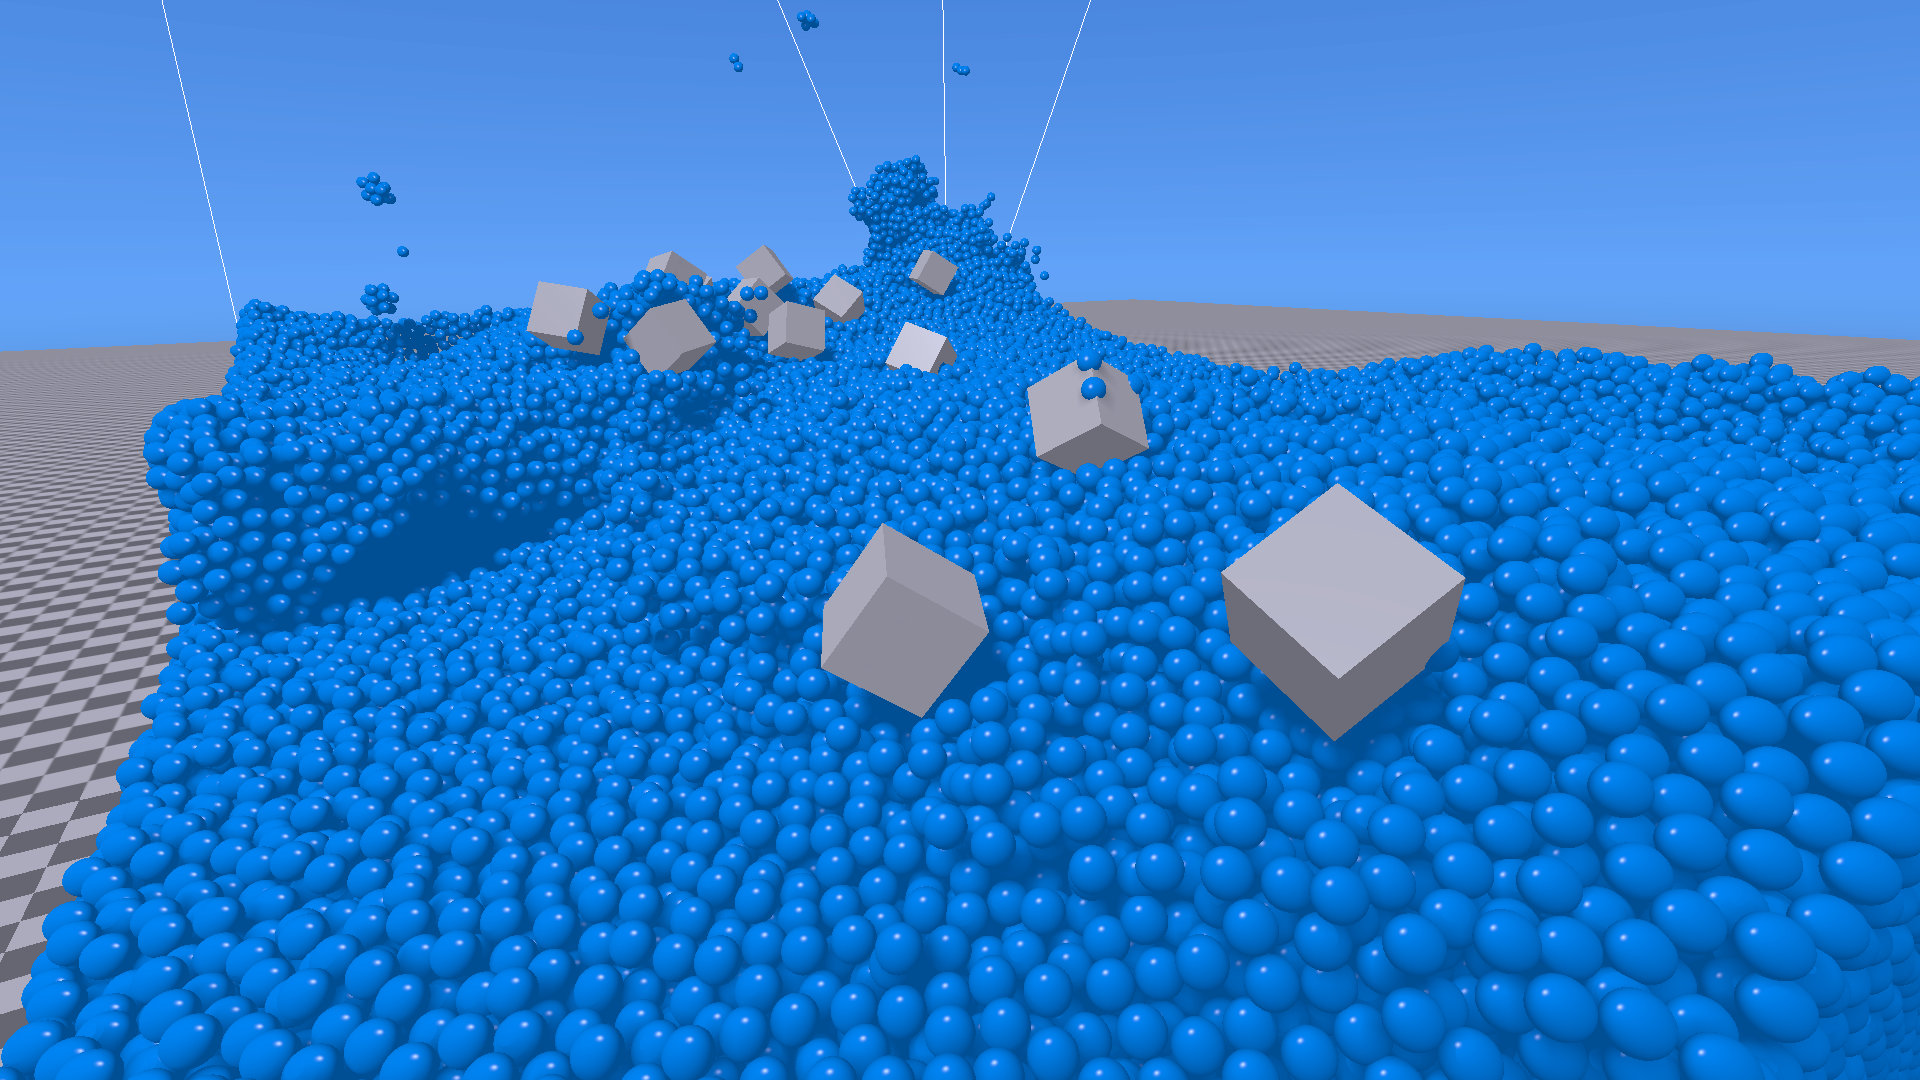
\includegraphics[height=.35\textheight]{agphys}
   	\end{figure}
\end{minipage}
\end{frame}

\frame{
	\frametitle{CUDA Course Overview}

	\begin{enumerate}
		\item The CUDA Programming Model (this lecture)
		\item Device Architecture and Parallel Communication
		\item Parallel Algorithms
		\item Profiling and Optimizing CUDA Code
	\end{enumerate}
}

\frame
{
	\frametitle{What is CUDA?}
	\begin{mdframed}
		CUDA is a \textbf{parallel computing platform} that allows developers to use the graphics processing unit for \textbf{general purpose processing} (GPGPU).
	\end{mdframed}
}

\frame{
	\frametitle{History of GPGPU}
\begin{table}
	\centering
		\color{gray}
		\ytl{2001}{GeForce 3 - First programmable shader pipeline with DirectX 8}
		\ytl{2001}{
		Larsen \& McAllister - first GPU matrix multiplication (8-bit) Hardware 	
	}
\ytl{2002}{
	Harris \& Coombe - Physically-Based Visual Simulation on Graphics Hardware 	
}
\end{table}

	\begin{figure}[!h]
	\begin{subfigure}{.3\textwidth}
		\centering
		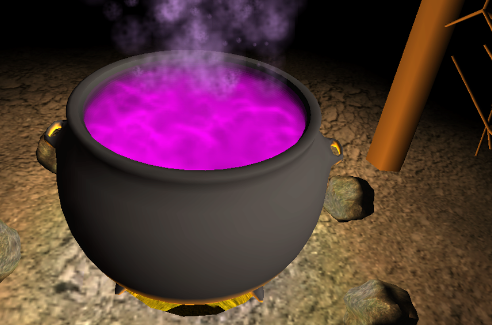
\includegraphics[height=.3\textheight]{phys1}
	\end{subfigure}%
	\begin{subfigure}{.3\textwidth}
		\centering
		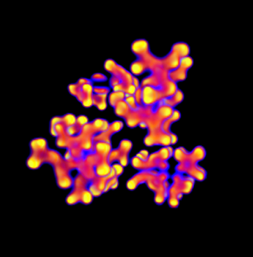
\includegraphics[height=.3\textheight]{phys2}
	\end{subfigure}
\begin{subfigure}{.3\textwidth}
	\centering
	
\includegraphics[height=.3\textheight]{phys3}
\end{subfigure}
\end{figure}
}



\frame{
	\frametitle{History of GPGPU}
	\begin{table}
		\centering
		\color{gray}
		\ytl{2002}{Programmable shaders in OpenGL 1.3 (as ARB extension)}
		\ytl{2002}{Purcell - Ray Tracing}
		\ytl{2003}{Bolz et al - Conjugate gradient}
		\ytl{2003}{Krueger et al - Fluid and cloud simulation}
	\end{table}
	
	\begin{figure}[!h]
		\begin{subfigure}{.3\textwidth}
			\centering
			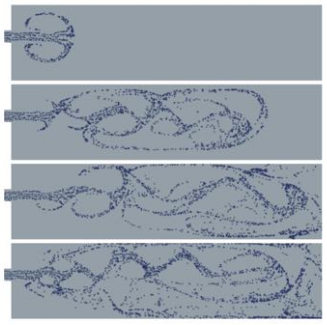
\includegraphics[height=.3\textheight]{phys6}
		\end{subfigure}%
		\begin{subfigure}{.3\textwidth}
			\centering
			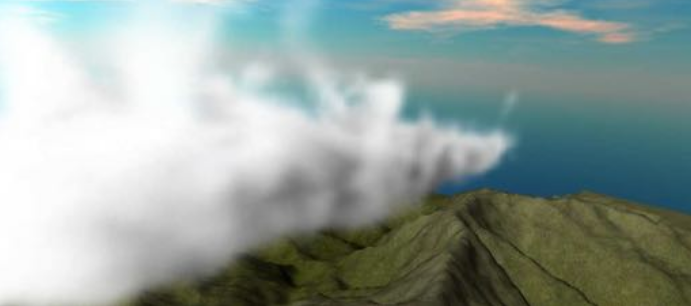
\includegraphics[height=.3\textheight]{phys4}
		\end{subfigure}
		\begin{subfigure}{.3\textwidth}
			\centering
			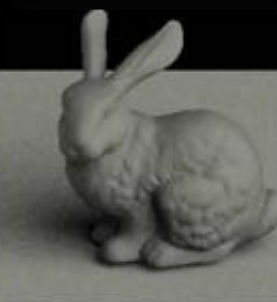
\includegraphics[height=.3\textheight]{phys5}
		\end{subfigure}
	\end{figure}
}

\frame{
	\frametitle{History of GPGPU}
	\begin{table}
		\centering
		\color{gray}
		\ytl{until 2007}{All GPGPU programs in vertex/fragment shaders}
		\ytl{2007}{Release of CUDA 1.0 - First GPGPU API}
		\ytl{2009}{OpenCL 1.0}
		\ytl{2009}{DirectCompute in DirectX 11}
		\ytl{2012}{OpenGL 4.2 compute shader}
	\end{table}
	
	\begin{figure}[!h]
		\begin{subfigure}{.2\textwidth}
			\centering
			
\includegraphics[height=.3\textheight]{cuda}
		\end{subfigure}%
		\begin{subfigure}{.2\textwidth}
			\centering
			
\includegraphics[height=.3\textheight]{opencl}
		\end{subfigure}
		\begin{subfigure}{.2\textwidth}
			\centering
			
\includegraphics[height=.3\textheight]{d11}
		\end{subfigure}
			\begin{subfigure}{.3\textwidth}
		\centering
		
\includegraphics[height=.3\textheight]{opengl}
	\end{subfigure}
	\end{figure}
}


\begin{frame} [fragile]
	\frametitle{CPU Parallel Programming}
	\textbf{CPU (C++ Threads)}
	\begin{itemize}
		\item Threads are launched using the C++ std lib
		\item Each thread can execute different code
		\item %
\begin{lstlisting} 
// Launch 1 thread that executes 'myFunction'
std::thread t1(myFunction);
\end{lstlisting}
	\end{itemize}
	\textbf{CPU (OpenMP)}
		\begin{itemize}
			\item Parallelize sections or loops
			\item Same code is run by multiple threads with different indices or TIDs
			\item %
\begin{lstlisting} 
#pragma omp parallel for num_threads(8)
for(int i = 0; i < N; ++i) {
	// ...
\end{lstlisting}
		\end{itemize}
\end{frame}


\begin{frame} [fragile]
	\frametitle{GPU Parallel Programming}

	\textbf{GPU (CUDA)}
		\begin{itemize}
			\item Requires special GPU functions (Kernels)
			\item Kernels are launched with multiple threads
			\item All threads from one launch execute the same code (the kernel)
			\item Each thread can compute its own unique thread id
			\item %
\begin{lstlisting} 
// Launch 1024 threads that execute 'myKernel'
myKernel<<<1,1024>>>();
\end{lstlisting}
			\item[$\rightarrow$] Similar idea to OpenMP
		\end{itemize}
\end{frame}




\begin{frame} [fragile]
	\frametitle{Sample Code Dependencies}
		\begin{itemize}
			\item Latest NVidia Graphics Driver \href{https://launchpad.net/~graphics-drivers/+archive/ubuntu/ppa}{[Ubuntu]}
			\item CUDA Toolkit 10.2 or newer \href{https://developer.nvidia.com/cuda-downloads}{[nvidia.com]}
			\item CMake 3.18 or newer \href{https://github.com/Kitware/CMake/tags}{[GitHub]}
			\item Eigen (latest version from git) \href{https://gitlab.com/libeigen/eigen}{[GitLab]}
		\end{itemize}
\end{frame}



\begin{frame}[fragile]
\frametitle{Run the Samples}
\begin{itemize}
	\item Download the samples and navigate to the code directory \href{https://github.com/darglein/saiga/tree/master/samples/cuda/helloCuda}{(Link @GitHub)}
	\item Run CMake 
\end{itemize}
\begin{lstlisting}[language=bash]
mkdir build && cd build
CXX=g++-9 CUDAHOSTCXX=g++-9 cmake ..
\end{lstlisting}
\begin{itemize}
	\item Compile and run
\end{itemize}
\begin{lstlisting}[language=bash]
make -j4 && ./hello_world
\end{lstlisting}

\begin{mdframed}[frametitle=Note:]
	The latest C++ compilers are usually not supported for CUDA host code.
\end{mdframed}
	
\end{frame}

\begin{frame}[fragile]
\frametitle{CUDA Hello World}
\begin{lstlisting}
// The __global__ keywort defines CUDA kernels!
__global__ void helloCudaKernel()
{
	printf("Hello from thread %d!\n", threadIdx.x);
}

int main(int argc, char *argv[])
{
	// Launch the kernel with 8 threads
	helloCudaKernel<<<1,8>>>();
	
	// Wait until completion
	cudaDeviceSynchronize();
	
	return 0;
}
\end{lstlisting}
\end{frame}

\begin{frame}[fragile]
\frametitle{CMake and CUDA}
	\begin{itemize}
	\item We recommend CMake version 3.18 and newer for the latest features

		\end{itemize}
\begin{lstlisting}[language=bash]
cmake_minimum_required(VERSION 3.18 FATAL_ERROR)
project ("Cuda Intro 1" VERSION 1.0.0 LANGUAGES CXX CUDA)

# CMake automatically compiles .cu file with NVCC
add_executable(hello_world hello_world.cu)

# Compile for Pascal and newer cards
set_property(TARGET hello_world 
	PROPERTY CUDA_ARCHITECTURES 52-virtual )
\end{lstlisting}
\end{frame}




\begin{frame}[fragile]
	\frametitle{Launch Arguments}
	\begin{itemize}
		\item The launch arguments define how many instances of the kernel are run on the GPU
\begin{lstlisting}
myKernel<<<num_blocks, threads_per_block>>>();
\end{lstlisting}
		\item The first parameter is the number of blocks
		\item The second parameter is the number of threads per block
	\end{itemize}
\end{frame}

\begin{frame}[fragile]
	\frametitle{Launch Arguments}
	\begin{itemize}
		\item Launch 1 block with 256 threads (256 threads total):
\begin{lstlisting}
myKernel<<<1,256>>>();
\end{lstlisting}
		\item Launch 8 blocks with 32 threads each (256 threads total):
\begin{lstlisting}
myKernel<<<8,32>>>();
\end{lstlisting}
	\end{itemize}
\end{frame}

\begin{frame}[fragile]
	\frametitle{Launch Arguments}
	The launch arguments can be 2- and 3-Dimensional. This makes distributing threads over grids (for example images) easier.
	\begin{itemize}
		\item Launch 2 blocks with 32x32 threads ($2 \cdot 32 \cdot 32 = 2048$ threads total):
\begin{lstlisting}
myKernel<<<2,dim3(32,32,1)>>>();
\end{lstlisting}
		\item Launch 2x2 blocks with 8x8 threads each ($2\cdot 2 \cdot 8 \cdot 8 = 256$ threads total):
\begin{lstlisting}
myKernel<<<dim3(2,2,1),dim3(8,8,1)>>>();
\end{lstlisting}
	\end{itemize}
\end{frame}



\begin{frame}[fragile]
\frametitle{Launch Arguments}

\begin{itemize}
	\item The current block id is:
\begin{lstlisting}
int blockId = blockIdx.x;
\end{lstlisting}
	\item The local thread Id (relative to the block) is:
\begin{lstlisting}
int tid = threadIdx.x;
\end{lstlisting}
	\item The block size is:
\begin{lstlisting}
int blockSize = blockDim.x;
\end{lstlisting}	
	\item In most kernels the global thread id is required:
\begin{lstlisting}
int global_tid = blockDim.x * blockIdx.x + threadIdx.x;
\end{lstlisting}
	\item \textbf{Note}: For 2-,3D arguments the y and z entry is used.
\end{itemize}
\end{frame}


\begin{frame}[fragile]
\frametitle{CUDA Hello World}
\begin{lstlisting}
// The __global__ keywort defines CUDA kernels!
__global__ void helloCudaKernel(int a)
{
	printf("Hello from thread (%d,%d). a = %d!\n", 
	   blockIdx.x, threadIdx.x, a);
}

int main(int argc, char *argv[])
{
	// Launch the kernel with 2 blocks, each 4 threads
	helloCudaKernel<<<2,4>>>(42);
	
	// Wait until completion
	cudaDeviceSynchronize();
	
	return 0;
}
\end{lstlisting}
\end{frame}


\begin{frame}[fragile]
\frametitle{Kernel Arguments}

\begin{lstlisting} 
myKernel<<<1,1024>>>(5, device_data, dt);
\end{lstlisting}

\begin{itemize}
	\item Kernel arguments are passed by value
	\item Automatically uploaded to GPU memory (only the value and not the data behind a pointer)
	\item Max size 256B (sum of all arguments)
	\item Never pass a pointer to CPU  memory!
\end{itemize}
\end{frame}


\begin{frame}[fragile]
	\frametitle{GPU Memory}
	Explicit allocation/deallocation:
	\begin{itemize}
		\item cudaMalloc, cudaFree
	\end{itemize}
	Explicit copy between host-device:
	\begin{itemize}
		\item cudaMemcpy
	\end{itemize}
	\textbf{We recommend to use the \textit{Thrust} library for memory management:}
\begin{lstlisting}
thrust::device_vector<float> device_data(200);
\end{lstlisting}

\begin{mdframed}[frametitle=Note:]
	Thrust is a C++ template library included in the CUDA toolkit. The syntax and functionality is similar to the C++ 11 standard library.
\end{mdframed}
	
\end{frame}


\begin{frame}[fragile]
	\frametitle{Particle Example}
	Task:
	\begin{enumerate}
		\item Allocate memory for particles
		\item Initialize particles and upload them to the GPU
		\item Integrate Position/Velocity of the particles
		\item Download result to the CPU
	\end{enumerate}
	
	\href{https://github.com/darglein/CudaTutorial/blob/master/1_Introduction/Code/simple_particle.cu}{Source @GitHub}
\end{frame}

\begin{frame}[fragile]
\frametitle{Particle Example (1.)}
\begin{lstlisting}
const int N     = 25;
const int steps = 3;
float dt        = 0.1;

// Allocate CPU and GPU memory
std::vector<Particle> particles(N);
thrust::device_vector<Particle> d_particles(N);
\end{lstlisting}
\end{frame}

\begin{frame}[fragile]
\frametitle{Particle Example (2.)}
\begin{lstlisting}
// Initialize on the CPU
for (Particle& p : particles)
{
    p.position = vec3::Zero();
    p.velocity = vec3::Random();
}

// Upload memory
thrust::copy(particles.begin(), particles.end(), d_particles.begin());
\end{lstlisting}
\end{frame}

\begin{frame}[fragile]
\frametitle{Particle Example (3.)}
\begin{lstlisting}
__global__ static void update(Particle* particles, int N, float dt)
{
    int tid = GlobalThreadId();
    if (tid >= N) return;
    Particle& p = particles[tid];
    p.position += p.velocity * dt;
    p.velocity += vec3(0, -9.81, 0) * dt;
}

// ...
for (int i = 0; i < steps; ++i)
{
    updateParticles<<<iDivUp(N, 128), 128>>>(
    	d_particles.data().get(), N, dt);
}
\end{lstlisting}
\end{frame}

\begin{frame}[fragile]
\frametitle{Particle Example (4.)}
\begin{lstlisting}
// Download
thrust::copy(d_particles.begin(), d_particles.end(), 
	particles.begin());

// Debug Print
for (Particle& p : particles)
{
    std::cout << p.position.transpose() << " " 
    	<< p.velocity.transpose() << std::endl;
}
\end{lstlisting}
\end{frame}

\begin{frame}[fragile]
	\frametitle{Blocks and Warps}
\begin{itemize}
\item Internally, a threadblock is further subdivided into \textbf{Warps} of 32 threads
\item For example after launching 2 blocks of 128 threads
\begin{lstlisting}
myKernel<<<2,128>>>();
\end{lstlisting}
\item Each block consists of 4 Warps ($4\cdot 32 = 128$)
\item And we have launched 8 Warps in total
\end{itemize}
\end{frame}

\begin{frame}[fragile]
	\frametitle{Blocks and Warps}
\begin{itemize}
	\item The block size should be a multiple of the Warp size
	\item All Threads in a warp \textbf{share the program counter} (Pascal and earlier)
	\item [$\rightarrow$] Excessive branching in warps should be avoided.
	\item [$\rightarrow$] High branching is usually called \textbf{warp divergence}.
\end{itemize}


\end{frame}


\frame{
	\frametitle{OpenGL Interoperability}
	%https://docs.nvidia.com/cuda/cuda-c-programming-guide/index.html#graphics-interoperability
	\begin{itemize}
		\item OpenGL resources (buffers and textures) can be \textbf{mapped} into the CUDA address space (\href{https://docs.nvidia.com/cuda/cuda-c-programming-guide/index.html\#graphics-interoperability}{Documentation})
		\item[$\rightarrow$] The resources can be read or written by kernels
	\end{itemize}
	Steps
	\begin{enumerate}
		\item Register the OpenGL resource once (\texttt{cudaGraphicsGLRegisterBuffer})
		\item Map the resource (\texttt{cudaGraphicsMapResources})
		\item Extract the device pointer (\texttt{cudaGraphicsResourceGetMappedPointer})
		\item Run your kernel
		\item Unmap the resource (\texttt{cudaGraphicsUnmapResources})
	\end{enumerate}
}


\begin{frame}[fragile]
\frametitle{CUDA Memcheck}
Checks for illegal memory accesses, unaligned reads/writes, ...
\begin{lstlisting}[language=bash]
cuda-memcheck ./helloWorld
\end{lstlisting}
Example Output:
\begin{lstlisting}[language=bash]
Invalid __global__ write of size 4
	at 0x000001b8 in segfault.cu:26:void oob<unsigned int=128>(int*, int)
	by thread (127,0,0) in block (15,0,0)
	Address 0x7f0717602000 is out of bounds
\end{lstlisting}
\textbf{Notes}
\begin{itemize}
\item Requires -G compiler flag for NVCC
\item Run cuda-memcheck before submitting your code
\end{itemize}

\end{frame}



\frame{
	\frametitle{Literature}
	%
	\begin{itemize}
		\item \href{http://cs.unc.edu/xcms/wpfiles/50th-symp/Harris.pdf}{Harris 2014, A Brief History of GPGPU}
		\item \href{http://www.markmark.net/cml/dl/HWW02_Harris_electronic.pdf}{Harris \& Coombe 2002, Physically-Based Visual Simulation on Graphics Hardware}	
		\item \href{https://docs.nvidia.com/cuda/}{Cuda Toolkit Documentation}
		\item \href{https://docs.nvidia.com/cuda/cuda-driver-api/}{CUDA driver API}
		\item \href{https://docs.nvidia.com/cuda/cuda-runtime-api/}{ CUDA runtime API}
		\item \href{https://docs.nvidia.com/cuda/thrust/index.html}{Thrust}
	\end{itemize}
	
}





\end{document}



